\section{\huge{Bonusopgaver}}
(til de flittige snapsedrikkere)


\subsection{Opgave 0}
Skriv en SML funktion, der finder det mindste tal, som er deleligt med alle
tal fra $1$ til $100$.


\subsection{Opgave 1}
Du har IP-adresseblokken 138.72.13.0/22. Hvor mange forskellige IP-adresser
råder du over? Angiv også den højeste og den laveste IP-adresse i dit råderum.


\subsection{Opgave 2}
Løs følgende ligningssystem:

\begin{align*}
A + B + 2C &= 21 \\
4A + 3D &= 40 \\
B + 2C + 4D &= 49 \\
A + 2B + 2C + 3D &= 58 \\
\end{align*}


\subsection{Opgave 3}
Omskriv tallet $154.7$ til dets 32-bit IEEE 754 repræsentation. Bliver der
mistet præcision?

\subsection{Opgave 4}

Find en tæt øvre og nedre asymptotisk grænse for følgende rekurrenseformel
\[
    T(n) = T(n/2) + T(n-1)\ .
\]
Antag at $T(n) = O(1)$ for $n < 2$.


\subsection{Opgave 5}
Du skal finde et nyt farveskema til \url{http://kantine.diku.dk}. Farveskemaet
skal være baseret på den mest brugervenlige farve. Hvilken af følgende er det?
\begin{enumerate}
    \item Marineblå
    \item Azurblå
    \item Ultramarin
    \item Kornblomst blå
\end{enumerate}
Fremstil en paper mock-up af den nye hjemmeside og foretag en fokusgruppe
undersøgelse med den relevante målgruppe. Rapporter dine resultater (ca.
40-50 sider) og giv referencer hvor nødvendigt.


\subsection{Opgave 6}
Giv et formelt bevis for følgende udsagn:
\[
    \forall x P(x)\lor \forall x Q(x)\Rightarrow \forall x \left(P(x)\lor
        Q(x)\right)\ .
\]


\subsection{Opgave 7}
Forklar hvad følgende INTERCAL kode gør. Er programmet høfligt nok? Er det
\emph{for} høfligt?
\begin{verbatim}
DO ,1 <- #13
PLEASE DO ,1 SUB #1 <- #238
DO ,1 SUB #2 <- #108
DO ,1 SUB #3 <- #112
DO ,1 SUB #4 <- #0
DO ,1 SUB #5 <- #64
DO ,1 SUB #6 <- #194
DO ,1 SUB #7 <- #48
PLEASE DO ,1 SUB #8 <- #22
DO ,1 SUB #9 <- #248
DO ,1 SUB #10 <- #168
DO ,1 SUB #11 <- #24
DO ,1 SUB #12 <- #16
DO ,1 SUB #13 <- #162
PLEASE READ OUT ,1
PLEASE GIVE UP
\end{verbatim}

Hvad er iøvrigt det fulde navn for programmeringssproget INTERCAL?

% Det er hello world

\subsection{Opgave 8}
Du er givet $n$ linjesegmenter, som udgør en pinball maskine, samt et
$x$-koordinat, hvor en pinball bliver smidt ned i maskinen. Bolden vil falde
nedad (negativ $y$-retning) indtil den rammer en af linjerne. Den følger
derefter linjen nedad indtil linjen slutter, hvorefter den falder videre ned.
Lav en algoritme, der beregner hvilket $x$-koordinat bolder falder ud af i
bunden. Det kan antages, at alle linjesegmenterne hælder, og at ingen af dem
overlapper. Se figuren herunder for et eksempel på hvordan bolden falder ned
igennem pinball maskinen.

Din algoritme skal køre $O(n\log n)$.

\begin{figure}[h!]
    \centering
    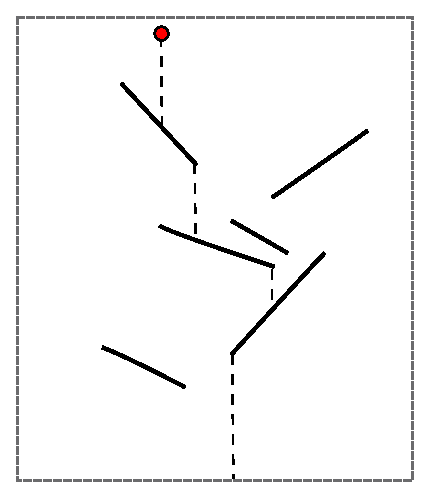
\includegraphics[width=0.7\linewidth]{figures/pinball.pdf}
    \caption{Eksempel på en bolds rute ned gennem pinball maskinen.}
    \label{fig:pinball}
\end{figure}

% Brug en sweepline fra top til bottom

\subsection{Opgave 9}

Lad $G$ være en plan, 3-regulær, bipartit graf, som er 3-vertex-connected.
Bevis eller modbevis at alle sådanne grafer $G$ indeholder en hamilton cycle.

\vspace{.1in}
\textbf{\emph{NB: Der udloddes en flaske snaps til den første som kommer op i baren med en korrekt besvarelse af denne opgave!}}

% Uløstproblem. "Barnette's Conjecture".
